\chapter{Authentifizierung}
\begin{itemize}
	\item \textbf{Authentifizierung:} Nachweis der \textit{Identität} eines Subjektes gegenüber einem anderen
	\item \textbf{Verifikation:} Identität wird bestätigt.
	\item \textbf{Identifikation:} Finden und Identifizieren eines Subjektes anhand von Referenzdaten (Fingerabdruck, Bild, ...)
\end{itemize}

\section{Voraussetzung für Authentifizierung}
\paragraph{Identifikationsmittel}
\begin{itemize}
	\item muss \textbf{eindeutig} sein
	\item kann \textbf{öffentlich} bekannt sein
\end{itemize}

\paragraph{Beweismittel}
\begin{itemize}
	\item meist unter Verschluss
	\item Beispiele: Passwort, private key, Fingerabdruck, preshared key, Iris, Chipkarte
\end{itemize}

\section{Realisierung der Authentifizierung}

\paragraph{Wissen}
\begin{itemize}
	\item Passwort
	\item PSK, SSH-Private-Key
	\item \textbf{Einfach anzugreifen}
	\item \textbf{Einfach zu ändern}
\end{itemize}

\paragraph{Besitz}
\begin{itemize}
	\item SmartCard
	\item Schlüssel
	\item \textbf{Kann entzogen werden!}
\end{itemize}
$\Rightarrow$ \textbf{Nicht (einfach) zu kopieren!}

\paragraph{Eigenschaften}
\begin{itemize}
	\item Biometrisches Merkmal einer Person (Iris, Fingerabdruck)
	\item False acceptence/reject
\end{itemize}
$\Rightarrow$ \textbf{nicht revozierbar!}

\subsection{Multi-Faktor-Authentifizierung}
Kombination von \textbf{min. 2} verschiedenen Beweismitteln \textbf{unterschiedlicher} Kategorien.\\
$\Rightarrow$ \textbf{Kompromittierung eines Faktors reicht nicht aus!}

\section{Ergebnis der Authentifizierung}
Das Subjekt erhält \textbf{Authentifizierungsbeweis}:
\begin{itemize}
	\item Session Cookie (Webbrowser)
	\item Session Key (TLS)
	\item Shell (Linux)
\end{itemize}
$\Rightarrow$ Identität wird auf \textbf{rechnerinternes} Objekt abgebildet.\\
$\Rightarrow$ \textbf{Schutz} des Authentifizierungsbeweises ist notwendig!

\section{Anforderungen an Authentifizierung}
\paragraph{Allgemeine Anforderungen}
\begin{itemize}
	\item Schutz des Authentifizierungsbeweises
	\item Schutz des Beweismittels
	\item Ergonomisch
	\item Einfach zu administrieren
\end{itemize}

\paragraph{Anforderungen bei Netzwerkauthentifizierung}
\begin{itemize}
	\item Keine sensiblen Daten über das Netz, im Klartext!
	\item Verhindern von Replay-Attacken!
	\item Verhindern von Man-in-the-Middle Angriffen!
\end{itemize}

\section{Authentifizierung mit Passwort}
\begin{itemize}
	\item idR. wird das Passwort im Rechner als \textbf{Hash} hinterlegt.
	\textbf{Salted Hash:} Passwort wird um Salt ergänzt, gehashed und mit dem hinterlegtem Wert verglichen.
	\item Salt:
	\begin{itemize}
	\item \textbf{Zufällige}, \textbf{pro Eintrag individuelle} Zeichensequenz
	\item Verhindert, dass identische Passwörter mit identischen Hashes abgespeichert werden
	\item Erschwert Wörterbuch- und Rainbowtable-Angriffe
	\end{itemize}
\end{itemize}

\section{Angriffe auf Passwortauthentisierung}
\paragraph{Angriffe}
\begin{itemize}
	\item Wörterbuchattacken
	\item Wörterbuchattacken auf Hashes
	\item Rainbow-Tables
\end{itemize}

\paragraph{Gegenmaßnahmen}
\begin{itemize}
	\item Langsame Hash-Algorithmen verwenden
	\item Salt
	\item Schutz der Hashes vor Auslesen
	\item Automatisches Sperren der Authentifizierung nach definierter Anzahl von Fehlversuchen
	\item Multifaktor-Authentifizierung 
\end{itemize}

\section{Biometrische Authentifizierung}
\begin{itemize}
	\item verwendet \textbf{individuelle Körpermerkmale} (Fingerabdruck, Irismuster, etc)
	\item Wesentliches Merkmal: biometrische Eigenschaften sind \textbf{immer leicht unterschiedlich}
\end{itemize}
\textbf{Ablauf:}
\begin{itemize}
	\item Einlernphase: mehrere Datenproben werden entnommen, daraus \textbf{Referenzdaten} erstellt
	\item 	Authentifizierung: neue Datenprobe wird genommen und mit Referenzdaten verglichen.\\ \textbf{Genügend Ähnlichkeit} $\Rightarrow$ authentifiziert.
\end{itemize}

\subsection{False-Reject vs. False-Accept}
\begin{figure}[H]
	\begin{center}
		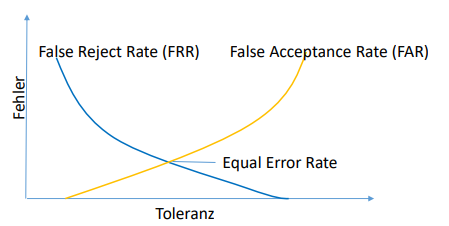
\includegraphics[scale=0.8]{Resources/FalseRejectFalseAcceptance.PNG}
		\caption{}
		\label{fig:FalseRejectFalseAcceptance.PNG}
	\end{center}
\end{figure}
\paragraph{False Reject Rate (FRR)}
\begin{itemize}
	\item Anteil der fälschlicherweise fehlgeschlagenen Authentifizierungsversuche
	\item Hohe FFR verringert Akzeptanz des Systems
\end{itemize}

\paragraph{False Acceptance Rate (FAR)}
\begin{itemize}
	\item Anteil der erfolgreichen
Authentifizierungsversuche, bei denen
fälschlicherweise eine andere Person
akzeptiert wird
	\item Hohe FAR verringert die Sicherheit deutlich!
\end{itemize}

\paragraph{Equal Error Rate}
\begin{itemize}
	\item Gibt die Toleranzschwelle an, bei der genauso viele Personen fälschlicherweise abgelehnt wie
fälschlicherweise akzeptiert werden (FAR=FRR)
	\item ist ein \textbf{Gütekriterium} für das biometrische Verfahren
	\item ist \textbf{nicht die Toleranzschwelle} mit der das System betrieben wird (normalerweise gilt: \textbf{FAR < FRR})
\end{itemize}

\section{Authentifizierung über Netzwerke}
\paragraph{zu Verhindern:}
\begin{itemize}
	\item Abhören
	\item Replay
	\item Man-in-the-Middle
	\item Übernehmen der authentifizierten Verbindung
	\item Ausfall des Authentifizierungssystems
\end{itemize}

\paragraph{Erreicht wird dies durch..}
\begin{itemize}
	\item Authentifizierung per Passwort (aber Verschlüsselte Verbindung)
	\item Zeitabhängige Passwörter / Einmalpasswörter
	\item Challenge-Response Authentifizierung
	\item Zertifikats- bzw. Public/Private-Key-Authentifizierung
\end{itemize}

\section{Einmalpasswörter}
Passwörter werden durch \textbf{Zähler} oder basierend \textbf{Zeitstempel} generiert.
Client und Server teilen gemeinsamen Schlüssel $K_A$ (individuell pro Client).
Der Schlüsselwert wird verwendet um:
\begin{itemize}
	\item aus einem Zählerwert $C$ und $K_A$ das Einmalpasswort zu bestimmen.
	\item aus dem aktuellen Zeitstempel $T$ und $K_A$ das Einmalpasswort zu bestimmen.
\end{itemize}
Server und Client berechnen unabhängig voneinander das Einmalpasswort. Die Authentifizierung ist erfolgreich, wenn dass Einmalpasswort übereinstimmt.\\
\\
\paragraph{Vorteile:}
\begin{itemize}
	\item Abgefangene Passwörter sind wertlos
	\item gemeinsamer Schlüssel $K_A$ kann clientseitig auf auslese-sicherer Hardware hinterlegt werden.
	\item Server erkennt Replay-Attacken
\end{itemize}
\paragraph{Nachteile:}
\begin{itemize}
	\item Gemeinsamer Schlüssel $K_A$ muss sicher auf Client und Server hinterlegt werden
	\item Ist $K_A$ bekannt können Einmalpasswörter vorrausberechnet werden. 
	\item Server hat Liste aller gemeinsamer Schlüssel
	\item Anfällig gegenüber Man-in-the-Middle.
	\begin{itemize}
		\item Separater Schutz gegen MiM notwendig!
		\item Typisch: Public-Private-Key-Auth des Server mittels SSL-Zertifikaten
	\end{itemize}
\end{itemize}

\section{Challenge-Response-Authentifizierung}
\begin{figure}[H]
	\begin{center}
		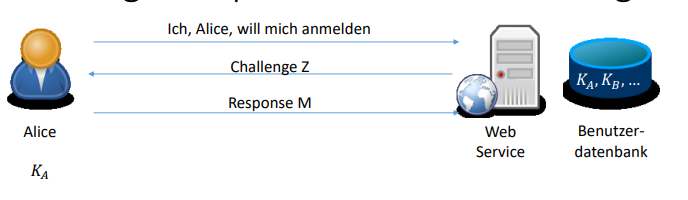
\includegraphics[scale=0.8]{Resources/ChallengeResponseAuth.png}
		\caption{}
		\label{fig:ChallengeResponeAuth.png}
	\end{center}
\end{figure}

\begin{enumerate}
	\item Alice schickt ihren Namen an den Server
	\item Server antwortet mit einer Nonce $Z$ (\enquote{Number used once}) an Alice
	\item Alice berechnet und schickt $M = Hash(K_A, Z)$ an den Server
	\item Server berechnet $M' = Hash(K_A, Z)$, falls $M' = M$ dann ist Alice authentifiziert.
	\item Alice und Server erzeugen gemeinsamen Session Key $K_S = KDF(K_A, Z)$
	\item Weitere Kommunikation wird mit $K_S$ verschlüsselt. $K_S$ ist der Authentifizierungsbeweis.
\end{enumerate}

\section{GSM-Authentifizierung}
Authentifizierung für eine hohe Anzahl von Teilnehmern. Zweck:
\begin{itemize}
	\item Missbräuchliche Verwendung des Mobilfunknetztes verhindern
	\item Abrechnung von Mobilfunknutzung
\end{itemize}
Implementierung: Challenge-Response-Auth: SIM-Karte enthält $K_A$, der nicht direkt ausgelesen werden kann.

\section{Private-Key-Authentifizierung}
Authentifizierung durch Nachweis des Besitz des Privaten Schlüssels.
\begin{figure}[H]
	\begin{center}
		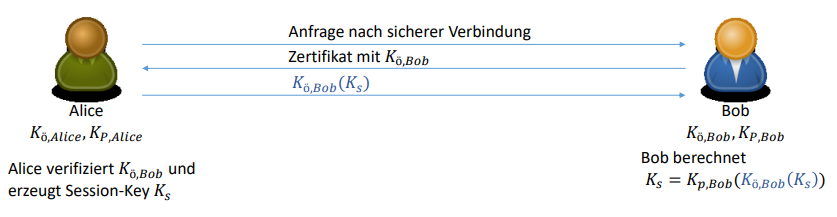
\includegraphics[scale=0.8]{Resources/PrivateKeyAuth.png}
		\caption{}
		\label{fig:PrivateKeyAuth.png}
	\end{center}
\end{figure}
\paragraph{Probleme:}
\begin{itemize}
	\item Session-Key $K_S$ wird über Netzwerk übertragen, und mit $K_pub, Bob$ verschlüsselt
	\item Wird $K_pri$ bekannt, können \textbf{aufgezeichnete Sessions im Nachhinein entschlüsselt werden}
	\item Jede Schwachstelle, die $K_pri$ freigibt ermöglicht Entschlüsselung aller vergangenen Sessions!
	\item Erneuerung des SSL-Zertifikats \textbf{tauscht Schlüssel idR nicht aus}
\end{itemize}

\paragraph{Abhilfe: Diffie-Hellman-Schlüsselaustausch}
\begin{figure}[H]
	\begin{center}
		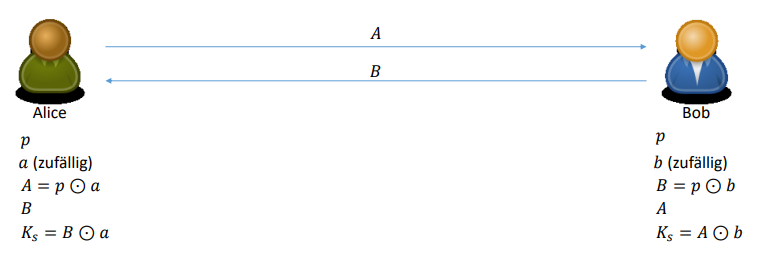
\includegraphics[scale=0.85]{Resources/DiffieHellman.png}
		\caption{Diffie-Hellman Schlüsselaustausch}
		\label{fig:DiffieHellman.png}
	\end{center}
\end{figure}
\begin{itemize}
	\item $K_S$ wird via DH-Algorithmus erzeugt.
	\item Anwendung bei SSL in Cipher-Suites: DHE (Diffie-Hellman Ephemeral) oder ECDHE (Elliptic Curve, DHE)
	\item \textbf{Perfect-Forward-Secrecy:} Kein nachträgliches Entschlüsseln von Sessions durch Bekanntwerden von $K_priv$ 
\end{itemize}

\section{x.509 Authentifizierung}
Authentifizierung mittels Zertifikaten:
\begin{itemize}
	\item Alice $\Rightarrow$ Bob: $Sign[K_{priv, A} \ , \ K_{pub, B}(K_S, Alice, Z,T)]$
	\item $K_{priv, A}$ private Key von Alice
	\item $K_{pub, B}$ public Key von Bob
	\item $K_S$ der Session-Key
	\item $Z$ eine Nonce (Replay Schutz)
	\item $T$ ein Zeitstempel (Replay Schutz)
\end{itemize}
\begin{enumerate}
	\item Alice ist authentifiziert, da Bob die \textbf{Signatur} von Alice prüft.
	\item Durch \textbf{Angabe der Identität} in den signierten Daten wird verhindert, dass sich ein MiM einschaltet und die Signatur ersetzt
	\item Die Kombination von $Z$ und $T$ dient als \textbf{Replay Schutz}: Der Server merkt sich für eine bestimmte Zeit alle Nonces und lehtn Auth ab, wenn eine Noce wiederverwednet wird.
\end{enumerate}

\section{FIDO-Alliance: U2F (Universal Second Factor)}
Standard von 2014 für zert-basierte Auth. via USB oder NFC-Token.

\paragraph{Initialisierung:}

\begin{itemize}
	\item Token erzeugt Schlüsselpaar für jede Site. Privater Schlüssel verlässt das Token nicht.
	\item Key-Handle identifiziert das Schlüsselpaar und muss die Information encodieren, für welche Website das Schlüsselpaar ist 
\end{itemize}
\begin{figure}[H]
	\begin{center}
		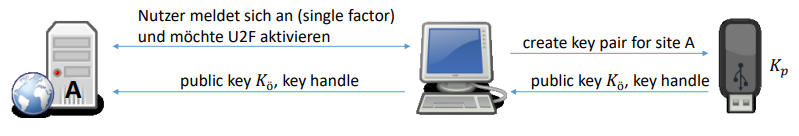
\includegraphics[scale=0.8]{Resources/FIDO1.png}
		\caption{}
		\label{fig:FIDO1.png}
	\end{center}
\end{figure}

\paragraph{Authentifizierung:}
\begin{itemize}
	\item Basierend auf dem Nutzernamen und der optionalen Auth mit Passwort oder PIN liefert der Server keyhandle und Noce
	\item Token Signiert Noce mit dem zum KeyHandle passenden $K_priv$. 
\end{itemize}

\begin{figure}[H]
	\begin{center}
		\includegraphics[scale=0.8]{Resources/Fido2}
		\caption{}
		\label{fig:Fido2}
	\end{center}
\end{figure}

\section{Single Sign On}
If someone steals my Laptop while I am logged inn, they can do everything but install drivers... 

\section{Probleme}
\begin{itemize}
	\item \textbf{einfache} Passwörter
	\item \textbf{wiederverwendete} Passwörter
	\item \textbf{unsicher gespeicherte} Passwörter
\end{itemize}

\section{Mapping der Authentifizierungsinformation}
\begin{itemize}
	\item Software/Dienst hält alle Auth-Infos
	\item Nutzer entsperrt diese Daten mit \textbf{Masterpasswort}
	\item \textbf{Vorteile:} 
	\begin{itemize}
		\item starke Servicepasswörter (generiert)
		\item nur \textbf{ein Passwort} zu merken (desshalb meistens besseres PW!) 
	\end{itemize}
	\item \textbf{Nachteile:}
	\begin{itemize}
		\item Ausfall des Mappingdienst sperrt sämtliche Zugriffe
		\item Sicherheit hängt an einem Passwort
	\end{itemize}
\end{itemize}

\section{Zentraler Authentifizierungsserver}
\begin{itemize}
	\item Nutzer authentifiziert sich bei zentralen Server (AS) und erhält ein Token.
	\item Token $\Rightarrow$ Auth bei Zielservern
\end{itemize}
\paragraph{Zu lösendes Problem:}
\begin{itemize}
	\item Token muss an die ID gebunden sein.
	\item Token darf auf dem Netzwerk nicht geklaut werden
	\item Server müssen verfizieren können, dass das Token vom korrektem Eigentümer verwendet wird.
\end{itemize}
$\Rightarrow$ Komplexe Sicherheitsprotokolle.
\paragraph{Vorteile:}
\begin{itemize}
	\item nicht clientgebunden
	\item zentrale Administration
	\item Hohe Sicherheit bei starker Anfangsauthentisierung
\end{itemize}

\paragraph{Nachteile:}
 \begin{itemize}
	\item Jeder Server muss das Protokoll können $\Rightarrow$ aufwendige Migration
	\item AS ist single point of falure
\end{itemize}

\section{Beispiel: Kerberos}
\begin{itemize}
	\item SSO-System (Single Sing On) mit symmetrischen Schlüsseln
	\item eingesetzt in Windows, Linux, NFS, SAP, Oracle ...
\end{itemize}

\subsection{Haupteigenschaften von Kerberos}
\begin{itemize}
	\item Zentrale Komponente hat Kenntnis aller Schlüssel (alle permanenten Schlüssel der Principal und Session-Keys)
	\item Datenelemente sind Ticket und Authenticator
	\item Authentifizierung erfolgt in drei Schritten
	\begin{enumerate}
		\item Ausstellung des Ticket Granting Ticket (TGT)
		\item Ausstellung des Zielserverticket
		\item Kommunikation mit dem Zielserver
	\end{enumerate}
\end{itemize}

\subsection{Grundbausteine von Kerberos}
\begin{itemize}
	\item Key Distribution Center (KDC):
	\begin{itemize}
		\item Authentifizierung (AS)
		\item Ticket Granting Service (TGS) 
		\item Authentifizierung, Tokenerstellung, Schutz der Tokens
	\end{itemize}
	\item Registry (sichere DB):
	\begin{itemize}
		\item enthält Namen und Schlüssel aller Benutzer 
	\end{itemize}
\end{itemize}

\subsection{Keberos Verfahren}
\begin{itemize}
	\item Kerberos verwendet \textbf{nur symmetrische Kryptographie}
	\item Server müssen um Kerberos-Komponente erweitert werden
	\item Clients müssen um Kerberos-Komponente erweitert werden
\end{itemize}

\subsection{Datenelemente von Kerberos}
\begin{itemize}
	\item \textbf{Schlüssel:}
	\begin{itemize}
		\item \textbf{für Personen:} Schlüssel werden aus Passwort abgeleitet. 
		\item \textbf{für Server:} starke Schlüssel werden zufällig generiert und mit Betriebssystemmitteln geschützt.
	\end{itemize} 
	\item \textbf{Tickets:}
	\begin{itemize}
		\item erlauben Nutzer (Prinzipal) die Authentifizierung an System oder Dienst
		\item Tickets transportieren Session-Keys
	\end{itemize}
	\item \textbf{Authentificator:}
	\begin{itemize}
		\item Binden Tickets an den Eigentümer
		\item bieten Replay-Schutz
	\end{itemize}
\end{itemize}

\subsubsection{Inhalt eines Kerberos-Tickets}
\begin{itemize}
	\item Zielservername
	\item verschlüsselt mit Schlüssel des Zielservers, ausgestellt durch TGS (Ticket Granting Service):
	\begin{itemize}
		\item Clientname
		\item Session-Key
		\item Gültigkeitsdauer 
	\end{itemize}
\end{itemize}

\subsubsection{Inhalt eines Kerberos-Authentificators}
\textbf{verschlüsselt mit Session-Key aus dem zugehörigem Ticket:}
\begin{itemize}
	\item Clientname
	\item Zeitstempel als Replay-Schutz
	\item Hashwert für mitgelieferte Daten
\end{itemize}
\textbf{Eigenschaften:}
\begin{itemize}
	\item Kann mehrmals verwendet werden	
	\item Authentificator wird jedes mal vom Client neu erzeugt
\end{itemize}

\subsection{Ablauf der Kerberos-Authentifizierung}
\begin{figure}[H]
	\begin{center}
		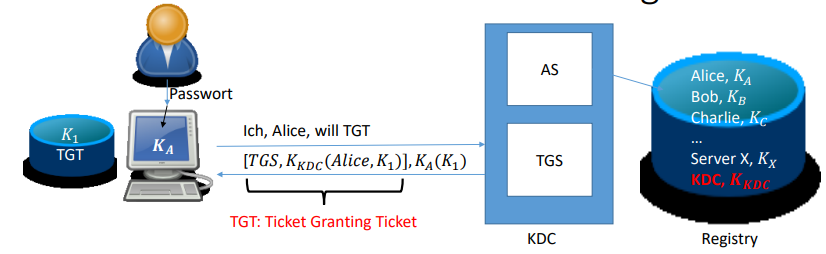
\includegraphics[scale=0.8]{Resources/AblaufKerberos1.png}
		\caption{}
		\label{fig:AblaufKerberos1.png}
	\end{center}
\end{figure}

\begin{enumerate}
	\item Alice frägt TGT an
	\item AS liest Alices Schlüssel aus der Registry aus
	\item KDC erzeugt ein Ticket für Alice zur Nutzung des TGS. $\Rightarrow$ TGT (\textbf{Ticket Granting Ticket})
	\item Alice gibt ihr Passwort ein, daraus wird $K_A$ berechnet
	\item Mit $K_A$ entschlüsselt Alice den Session-Key $K_1$ 
	\item Alice speichert $K_1$ und das TGT lokal
\end{enumerate}

\begin{figure}[H]
	\begin{center}
		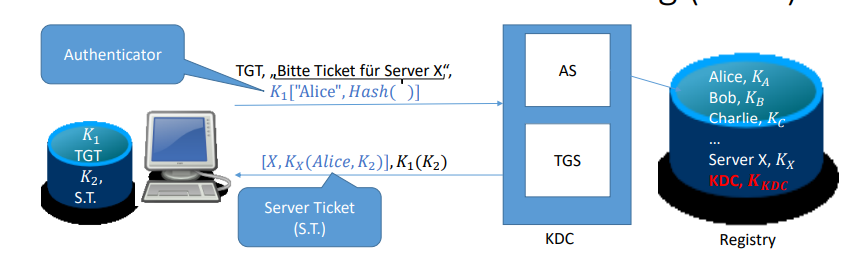
\includegraphics[scale=0.8]{Resources/AblaufKerberos2.png}
		\caption{}
		\label{fig:AblaufKerberos2.png}
	\end{center}
\end{figure}

\begin{enumerate}
	\item Alice schickt TGT mit Anfrage nach Server-Ticket an TGS.
	\item TGS kann TGT entschlüsseln, liest daraus den Session-Key $K_1$ und prüft damit den Authentificator $\Rightarrow$ Anfrage kann nur von Alice kommen
	\item TGS schickt Server Ticket und zusätzlich den Session-Key $K_2$ verschlüsselt für Alice
	\item Alice speichert Server Ticket und den Session Key $K_2$
\end{enumerate}

\subsection{Zugriff auf den Server}
\begin{figure}[H]
	\begin{center}
		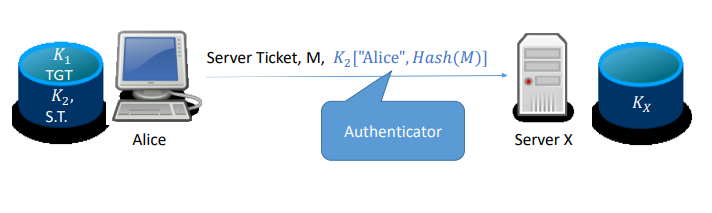
\includegraphics[scale=0.8]{Resources/KerberosZugriff.png}
		\caption{}
		\label{fig:KerberosZugriff.png}
	\end{center}
\end{figure}
\begin{itemize}
	\item Alice schickt Server Ticket und Authentificator an Server
	\item Server kann mit $K_X$ das Serverticket entschlüsseln und mit dem darin enthaltenen $K_2$ Authentificator von Alice überprüfen $\Rightarrow$ Nachricht $M$ ist authentisch von Alice!
	$K_2$ ist Authentifizierungbeweis von Alice für $X$ 
\end{itemize}

\subsection{Interdomain-Authentifizierung}
Wenn sich zwei Key-Distribution-Center $KDC_1$ und $KDC_2$ gegenseitig als Server eingetragen haben dann:
\begin{itemize}
	\item kann sich ein Nutzer von $KDC_1$ ein TGT für $KDC_2$ besorgen
	\item mit diesem TGT kann sich der Nutzer aus der Domäne von $KDC_1$ dann via $KDC_2$ Server Tickets für Server der Domäne von $KDC_2$ 
	\item Interdomain-Auth kann auch einseitig erfolgen ($KDC_1$ stellt TGTs für $KDC_2$ aus, aber nicht umgekehrt)
\end{itemize}

\subsection{Stärken und Schwächen von Kerberos}
\paragraph{Stärken}
\begin{itemize}
	\item Protokoll ist gut analysiert (da alt)
	\item clientunabhängigies SSO bei allen Teilnehmern einer Domäne
	\item flexibles und erweiterungsfähiges Protokoll
\end{itemize}

\paragraph{Schwächen}
\begin{itemize}
	\item Bei menschlichen Nutzern kann die Auth-anfrage für Passwortattacken genutzt werden (Key wird aus Passwort abgeleitet)
	\item KDC hat keine Zustandsinformationen (Logoff nur durch Ablauf des Tickets)
	\item KDC muss absolut vertrauenswürdig sein (ansonsten Golden Ticket möglich!)
	\item Client muss sicher sein
	\item keine Rechteverwaltung
\end{itemize}

\section{Shibboleth Authentifizierung}
\begin{figure}[H]
	\begin{center}
		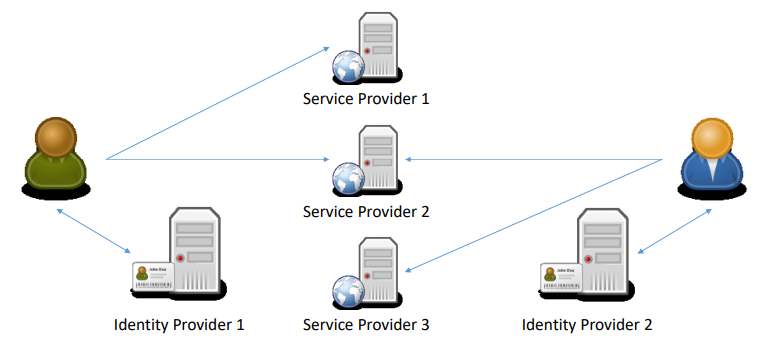
\includegraphics[scale=0.8]{Resources/ShibbolethAuth}
		\caption{}
		\label{fig:ShibbolethAuth}
	\end{center}
\end{figure}
Es gibt \textbf{Identitiy Provider (IdP)} und \textbf{Service Provider (SP)}.
Ablauf des Single-Sign-ONs (SSO):
\begin{enumerate}
	\item Client möchte Zugriff auf die Website
	\item Wenn dort nicht authentifiziert $\Rightarrow$ Umleitung auf den IdP (auch mehrere IdPs möglich)
	\item Bei IdP wird Auth durchgeführt
	\item Mit Bestätigung der Auth (Assertion) wird erneut der Service-Provider kontaktiert.
	$\Rightarrow$ bei weiteren SPs ist kein erneutes Login möglich
	\item IdP kann auch servicesperzifische Attribute an den SP weiterreichen.
\end{enumerate}
Existenz von Sessions wird durch entsprechende Cookies im Browser bestätigt.

\section{OAuth}
\begin{itemize}
	\item eigentlich ein \textbf{Authorisierungs}-Protokoll, kann aber zur \textbf{Authentifizierung} eingesetzt werden (?)
	\item Webanwendung will Zugriff auf die Ressourcen einer anderen Webanwendung (zB. Facebook-Pic auf Stackexchange)
	\item mit OAuth: Stackexchange kann mit Zustimmung des Facebook-Nutzers eine genau definierte Teilmenge der Nutzerrechte erhalten
\end{itemize}

\subsection{Rollen in OAuth}
\begin{itemize}
	\item \textbf{Resource Owner (auch End-User)}: entscheidet über Art und Umfang der Zugriffsberechtigungen
	\item \textbf{Resource Server:} im Besitz der Ressourcen. Er gewährt Zugriff, wenn \textbf{Access Token} präsentiert wird.
	\item \textbf{Client:} Webanwendung, die auf geschützte Ressource zugreifen will.
	\item \textbf{Auth-Server:} Server \textbf{authentifiziert} Client und übergibt im daraufhin das entsprechende Access-Token.
\end{itemize}

\subsection{Ablauf von OAuth}
\begin{figure}[H]
	\begin{center}
		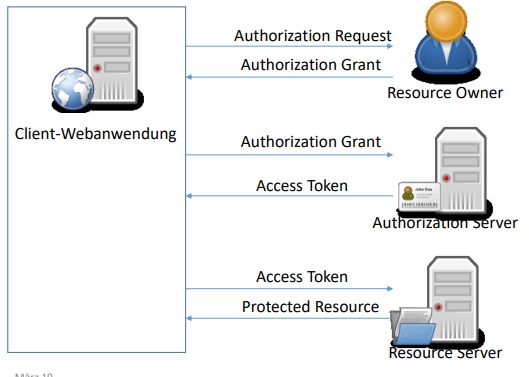
\includegraphics[scale=0.8]{Resources/OAuth}
		\caption{}
		\label{fig:OAuth}
	\end{center}
\end{figure}
\begin{itemize}
	\item Alle Verbindungen über \textbf{https}
	\item Der Authorization-Request kann indirekt über den Authorization-Server erfolgen
\end{itemize}

\subsection{OAuth-Flow}
\begin{figure}[H]
	\begin{center}
		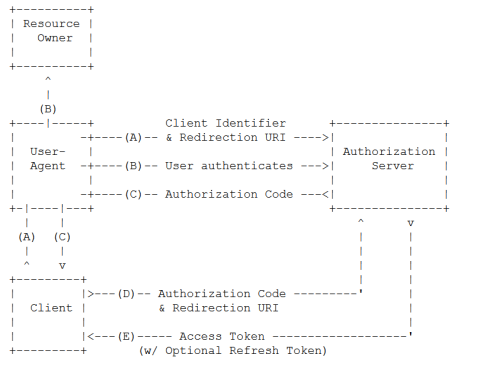
\includegraphics[scale=0.8]{Resources/OAuthFlow}
		\caption{}
		\label{fig:OAuthFlow}
	\end{center}
\end{figure}
\begin{itemize}
	\item empfohlene Abweichung vom ursprünglichem Flow für den Fall, dass es sich bei dem Client ebenfalls um eine Webanwendung handelt.
	\item Client und Authorization-Server müssen die Möglichkeit haben, im Browser einen \textbf{redirekt} anzustoßen.
\end{itemize}
























